\documentclass[../main.tex]{subfiles}


\begin{document}
\raggedright
The purpose of the project was to produce a system which will allow the students, secretary and the scrutiny panel to efficiently and securely store and access Extenuating Circumstance Forms as well as allow other staff members to access the simplified version of the students circumstance. Each of the following describes the requirement as well as the results achieved. 

\subsubsection{Mobile First}
Being coded in Bootstrap 4\cite{bootstrapfour} the system follows a mobile first coding approach which allows the website to be easily accessed on any mobile devices(Smart phones, iPads or laptops) with full functionality. Students can apply for extenuating circumstances at the comfort of their home in cases where their circumstance does not allow them to move out just to submit a printed form to the office. Figure \ref{fig:mosbilesystem} shows the system running on a Heroku Server and accessed on a mobile device as a Student trying to create a new Extenuating Circumstance Application. All panels including the Secretary Panel are mobile friendly and so can be accessed with the smallest smart phone. 

\begin{figure}[H]
        \center{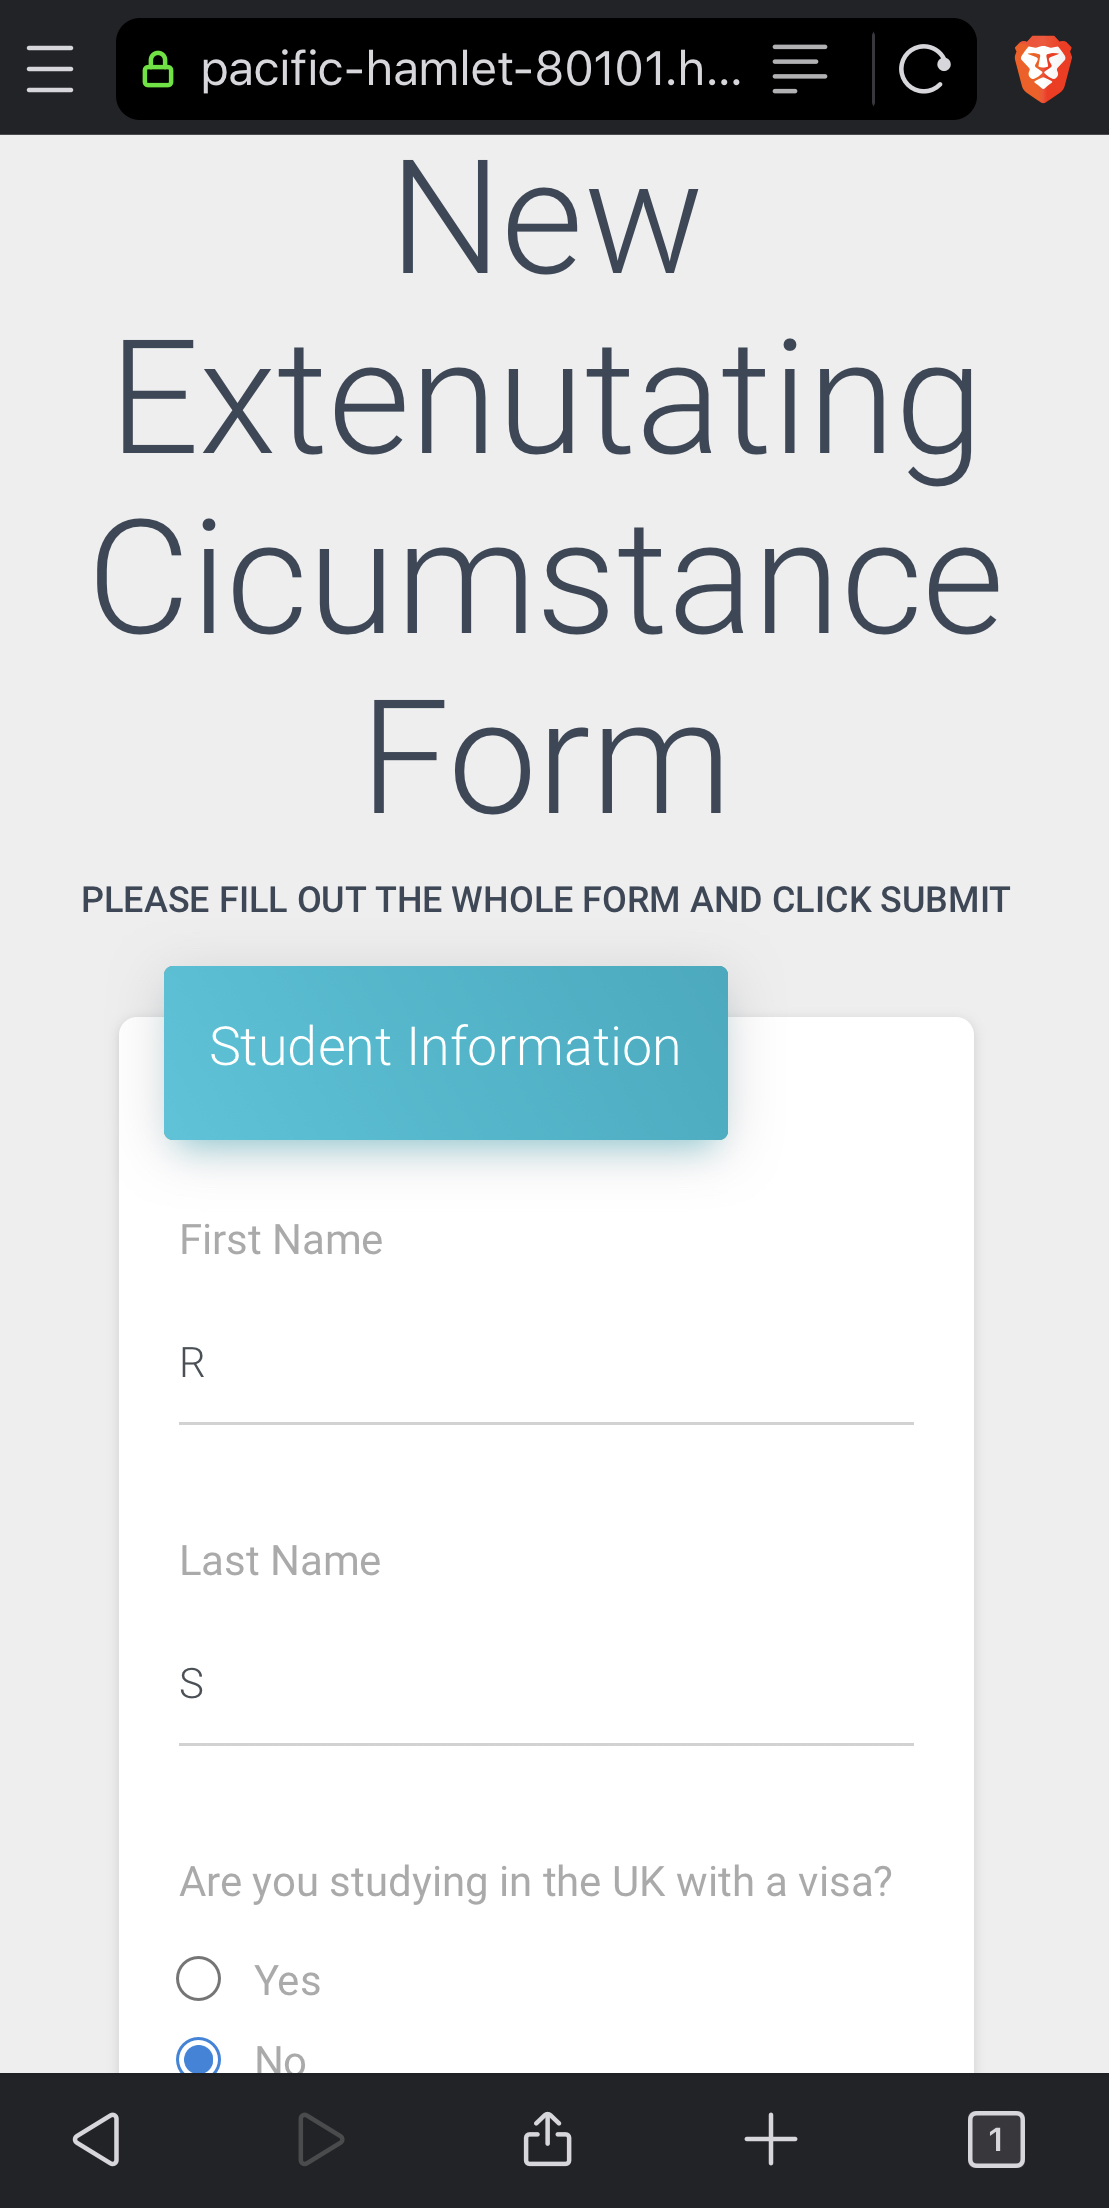
\includegraphics[scale=0.17]
        {images/mobiledevice.jpg}}
        \caption{\label{fig:mosbilesystem} Screenshot of the system running on a mobile device}
      \end{figure}
      
      
\subsubsection{Organised Data}
One of the issues with the previous system was the processing of data. A lot of data would be need to be duplicated which leaded to unorganised data records. Students would submit multiple forms at times with either a different circumstance or the same one which would again lead to improper data storage. With the Django system the data is well organised and easily accessible. Data is stored in tables with the ability to search for specific records and view past submissions as well.  Figure \ref{ecfstudenttable} and \ref{ecfsectable} show extenuating circumstance forms for both Students as well as what the Secretary and Scrutiny Panel would see. The status of the form allows all stakeholders to remain informed and students avoid multiple forms filled with the same data. The search field allows sorting and filtering through the forms extremely easily when searching for students, specific forms or status search. 

\begin{figure}[H]
        \center{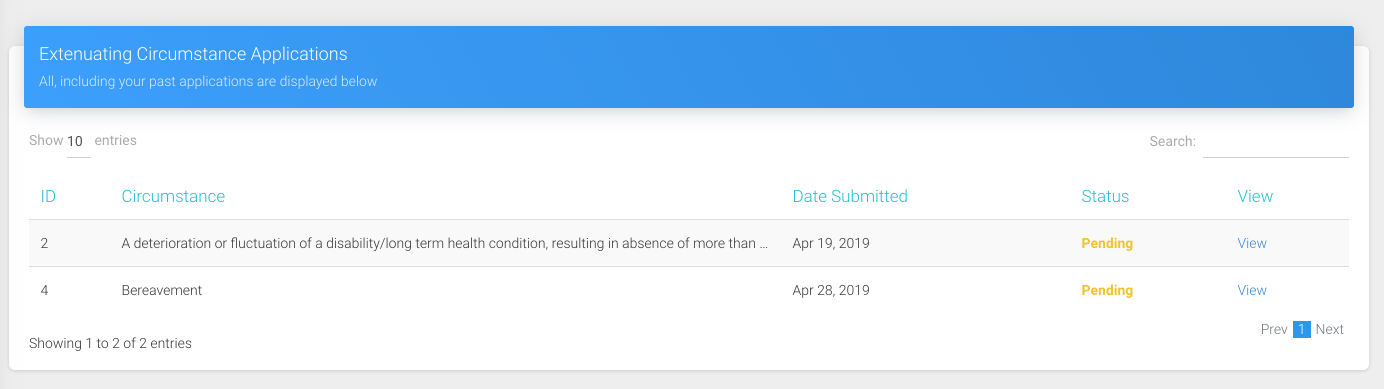
\includegraphics[scale=0.7]
        {images/ecfstudenttable.png}}
        \caption{\label{fig:ecfstudenttable} \textbf{Student Panel} Submitted Forms}
      \end{figure}
 
\begin{figure}[H]
        \center{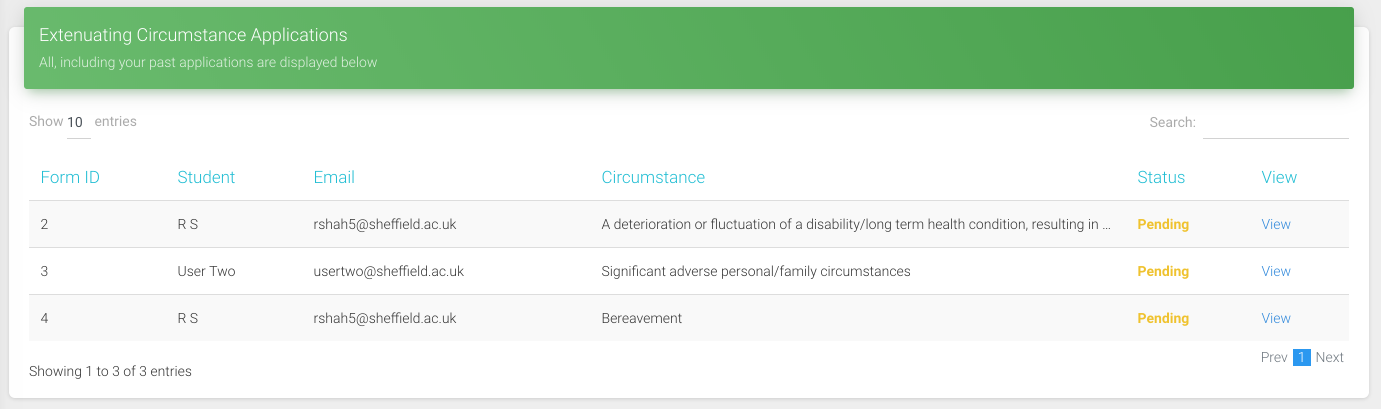
\includegraphics[scale=0.7]
        {images/ecfsectable.png}}
        \caption{\label{fig:ecfsectable} \textbf{Secretary/Scrutiny Panel} Submitted Forms}
      \end{figure}

\subsubsection{Security}      

\end{document}
